%% ID: lifting_rod
%% TITLE: Lifting a Rod
%% TYPE: question
%% QUESTIONTYPE: numeric
%% CONCEPTS: energy, eq_of_motion_diff, newtonii, resolving_vectors, vectors, moments
%% VIDEOS: 
%% LEVEL: 5
%% TOPIC: mechanics/dynamics
%% ORDER: 6

\begin{problem}[IntA1987APIQ1l] %Requires moments, work, power, simple pendulum, SHM
{\begin{enumerate}
	\item A non-uniform rod of mass \valuedef{m}{200}{kg} and length \valuedef{l}{10.0}{m} has its centre of mass \valuedef{d}{4.0}{m} from one end. It is supported horizontally by two vertical ropes which are attached to points \valuedef{s}{1.0}{m} from each end. Calculate the tension in each rope.
	\item The rod is raised by accelerating it at \valuedef{a}{0.20}{m\,s\sup{-2}} to a speed \valuedef{v}{0.60}{m\,s\sup{-1}}, which remains constant until the total height gained is \valuedef{h}{12.0}{m}. Calculate:
	\begin{enumerate}
		\item the sum of the tensions in the ropes when the rod is accelerating,
		\item the sum of the tensions in the ropes when the rod is moving up at a steady speed,
		\item the power required when lifting the rod at \vari{v},
		\item the distance for which the rod was accelerating and the distance for which it moved at \vari{v},
	\end{enumerate}
	\item Using the above, or otherwise, find the work done raising the rod in terms of \vari{m}, \vari{v} and \vari{h}. Comment on the value.
\end{enumerate}
}
{\stress{Adapted with permission from UCLES, A Level Additional Physics, November~1987, Paper~1, Question~1.}}
{\begin{enumerate}
	\item A diagram should always be the first step, showing the forces and key distances involved, as in Figure \ref{fig:Dynamics_rod_forces}. It is also best to remain in symbols for as long as possible; it allows dimension checking at the end.

\begin{figure}[h]
\centering
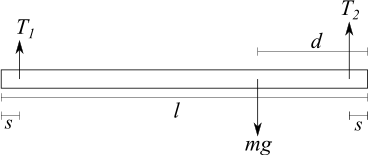
\includegraphics[width=0.5\textwidth]{../../../figures/Dynamics_rod_forces.svg}
\caption{}\label{fig:Dynamics_rod_forces}
\end{figure}

To find the tensions, we need to consider the moments about the two points where the ropes are attached, since this removes one tension from the equations each time. The rod is in equilibrium, so the total moment about any point must be zero. Thus taking moments about the point where \vari{T_{1}} acts will allow \vari{T_{2}} to be found and vice versa. The moments about the point \vari{T_{2}} acts:
\begin{align*}
(T_{1})(l - 2s) - (mg)(d - s) = 0 
\end{align*}
\begin{align*} 
T_{1} &= \frac{mg(d - s)}{l - 2s} \\ 
&= \frac{(200 \times 9.8)(4 - 1)}{(10 - 2)} \\
 &= \mbox{\quantity{735}{N}}
 \end{align*}
where the trickiest part is working out the distance to the point where the forces act.
Repeating the process to find \vari{T_{2}} gives:
\begin{align*}
(T_{2})(l - 2s) - (mg)(l - d - s) = 0 
\end{align*}
\begin{align*} T_{2} &= \frac{mg(l - d - s)}{l - 2s} \\ 
&= \frac{(200 \times 9.8)(10 - 4 - 1)}{(10 - 2)} \\ 
&= \mbox{\quantity{1225}{N}}
\end{align*}
and a quick check that the net force on the rod is zero: \valuedef{T_{1} + T_{2} - mg}{0}{} so check for our calculated values \vari{735 + 1225 - (200 \times 9.8)} $=$ \valuedef{1960 - 1960}{0}{N} as required.
	\item There are multiple ways to attempt each of the questions here, but all produce the same answers:
	\begin{enumerate}
		\item The sum of the tensions when the rope is accelerating can be found using \valuedef{\vtr{F}}{m\vtr{a}}{} and considering the net force:
	\begin{equation*}
	 F_{\text{tot}} = ma = T_{\text{tot}} - mg 
	 \end{equation*} 
	 and so the total of the tensions is 
	 \begin{align*} T_{\text{tot}} &= ma + mg \\ 
	 &= m(a + g) \\ &= (200)(0.2 + 9.8) \\ 
	 &= \mbox{\quantity{2000}{N}{} }
	 \end{align*}
		\item When the rod is moving at a constant speed, the net force must be zero and so we have the same situation as in the first part of the question. Another way of looking at it is that the acceleration is zero (\vari{a}{0}{m\,s\sup{-2}}) and so using the formula above we find that, as in the first part, the total of the tensions is \vari{mg}, as expected. This is because all inertial frames of reference (frames which are not accelerating) are equivalent and we could move into the frame of the moving rod, where the rod appears stationary but with the same forces acting on it. In order to give a consistent answer in both cases, a constant velocity cannot make a difference.
		\item The power required when lifting the rod is given by the equation \vari{P} $=$ \valuedef{\vtr{F} \cdot \vtr{v}}{Fv}{} where \vari{F} is as before, and \vari{v} is the speed in the direction the force is acting. Using this, we find:
	\begin{equation*} 
	P = Fv = (mg)(v) = (200 \times 9.8)(0.6) = \mbox{\quantity{1176}{W}} 
	\end{equation*}
This could also have been found another way; since the speed is constant, the power is the total energy required divided by the time taken to use that energy. Calling the distance moved at the constant speed \vari{s_{2}}:
	\begin{equation*} 
	P = \frac{E_{\text{used}}}{\Delta t} = \frac{mgs_{2}}{\Delta t} = mg\left(\frac{s_{2}}{\Delta t}\right) = mgv 
	\end{equation*} 
	as before.
		\item To find the two distances involved, we can simply use SUVAT. Call the distance moved whilst accelerating \vari{s_{1}}, and that moved whilst at a constant speed \vari{s_{2}}. The equation we need is \valuedef{v^{2}}{u^{2}+2as}{} where \valuedef{u}{0}{m\,s\sup{-1}}:
	\begin{align*} 
	s_{1} &= \frac{v^{2} - u^{2}}{2a} = \frac{v^{2}}{2a} \\ 
	&= \frac{(0.6)^{2}}{2(0.2)} = \mbox{\quantity{0.9}{m}}
	\end{align*}
and then \vari{s_{2}} is simply \vari{h - s_{1}} $=$ \valuedef{h - \frac{v^{2}}{2a}}{11.1}{m}.
	\end{enumerate}

\item We need to use the formula \vari{W} $=$ \valuedef{\vtr{F} \cdot \vtr{x}}{Fd}{} where \vari{F} is the magnitude of the force \vari{\vtr{F}} and d is the distance moved in the direction of the force. There are two sections to the motion; those when the rod is accelerating and the tension is \vari{T_{\text{tot}}} and that when it is moving at a constant speed, with tension $T = T_{1} + T_{2}$, and the total work is the sum of these two.
	\begin{align*} 
	W &= (T_{\text{tot}})(s_{1}) + (T)(s_{2})  \\ 
	&= \left[m(a + g)\right]\left[\frac{v^{2}}{2a}\right] + \left[mg\right]\left[h - \frac{v^{2}}{2a}\right] \\ 
	&= \frac{mav^{2}}{2a} + \frac{mgv^{2}}{2a} + mgh - \frac{mgv^{2}}{2a} \\ 
	&= \frac{1}{2}mv^{2} + mgh 
	\end{align*}
It should be clear that this is simply the sum of the kinetic and gravitational potential energy the rod gained as it was lifted; the work done by the ropes was the only way the rod could have gained energy, so an energy argument could have been used here instead.
\end{enumerate}}
\end{problem}